\section{Results}
\label{sec:results}

This section first gives an overview of a typical editorial process in the setting of scholarly communication. Then, the potential
for hybrid intelligent systems (with a focus on adaptability) as part of the editorial process is discussed. Finally, we derive two
hypotheses and subject them to qualitative feedback from a group of students in business information systems ($n = 25$).

\subsection{The Editorial Process}

A simplified, typical editorial process for a manuscript submitted to a journal -- from writing the manuscript to the final decision of
acceptance or rejection -- is shown in Figure ~\ref{fig:bpmnEditorialProcess}. The process includes at least three parties: the author who
writes the manuscript, the editor of the journal (or conference chair) that coordinates the peer-review process, and the peer-reviewers
that review and comment on a manuscript. For some journals the editor could be two persons: an academic editor, such as an \textit{Editor-in-Chief},
taking the decisions on manuscripts after peer-review, and an internal editorial staff coordinating the editorial process.

The typical editorial process involves several steps that must be completed in a particular order. First, the author writes the manuscript
with the research results. Once the manuscript is complete, the author searches for an appropriate journal to submit it to. Next, the author
formats the manuscript according to the specific instructions of the chosen journal (i.e., as a Microsoft Word or \LaTeX~document). The author
then submits the manuscript files to the journal for consideration and peer-review. 

Once the journal receives the manuscript, the editor performs a desk review to assess whether the manuscript meets the journal's requirements
and stated scope. If the editor finds that the manuscript could be a good fit for the journal, they will search for potential reviewers who
have expertise in the manuscript's subject. Depending on the journal and publisher, this task could be performed by the editorial staff of
the journal or by an external academic editor. In cases where the editor is an academic editor, they will typically search for reviewers
themselves. In cases where the editor is an internal editorial staff, they will typically use a reviewer recommendation system to search
for potential reviewers. Reviewer candidates are typically selected based on their expertise, previous publications, and after checking 
their conflicts of interests (e.g., if they have co-authored a paper with the author in the past). The editor will then invite reviewers
that passed the screening to evaluate the manuscript, i.e., invite them to peer-review the manuscript. If the reviewers accept the invitation,
they will be granted access to the manuscript, read it and write a review report that details their feedback and recommendations (typically
split into a part addressed to authors, and another part addressed to the editors of the journal). 

After all review reports have been received, the editor will read and assess each one. Based on the reviews, the editor will make a first
decision on whether to accept, reject, or request revisions to the manuscript. If revisions are required, the author will revise the manuscript
according to the review reports and asked to resubmit the revised version to the journal. The editor will then check the revised manuscript
and make a final decision on whether to accept it for publication in the journal.

\begin{landscape}
    \begin{figure*}[htb]
        \centering
        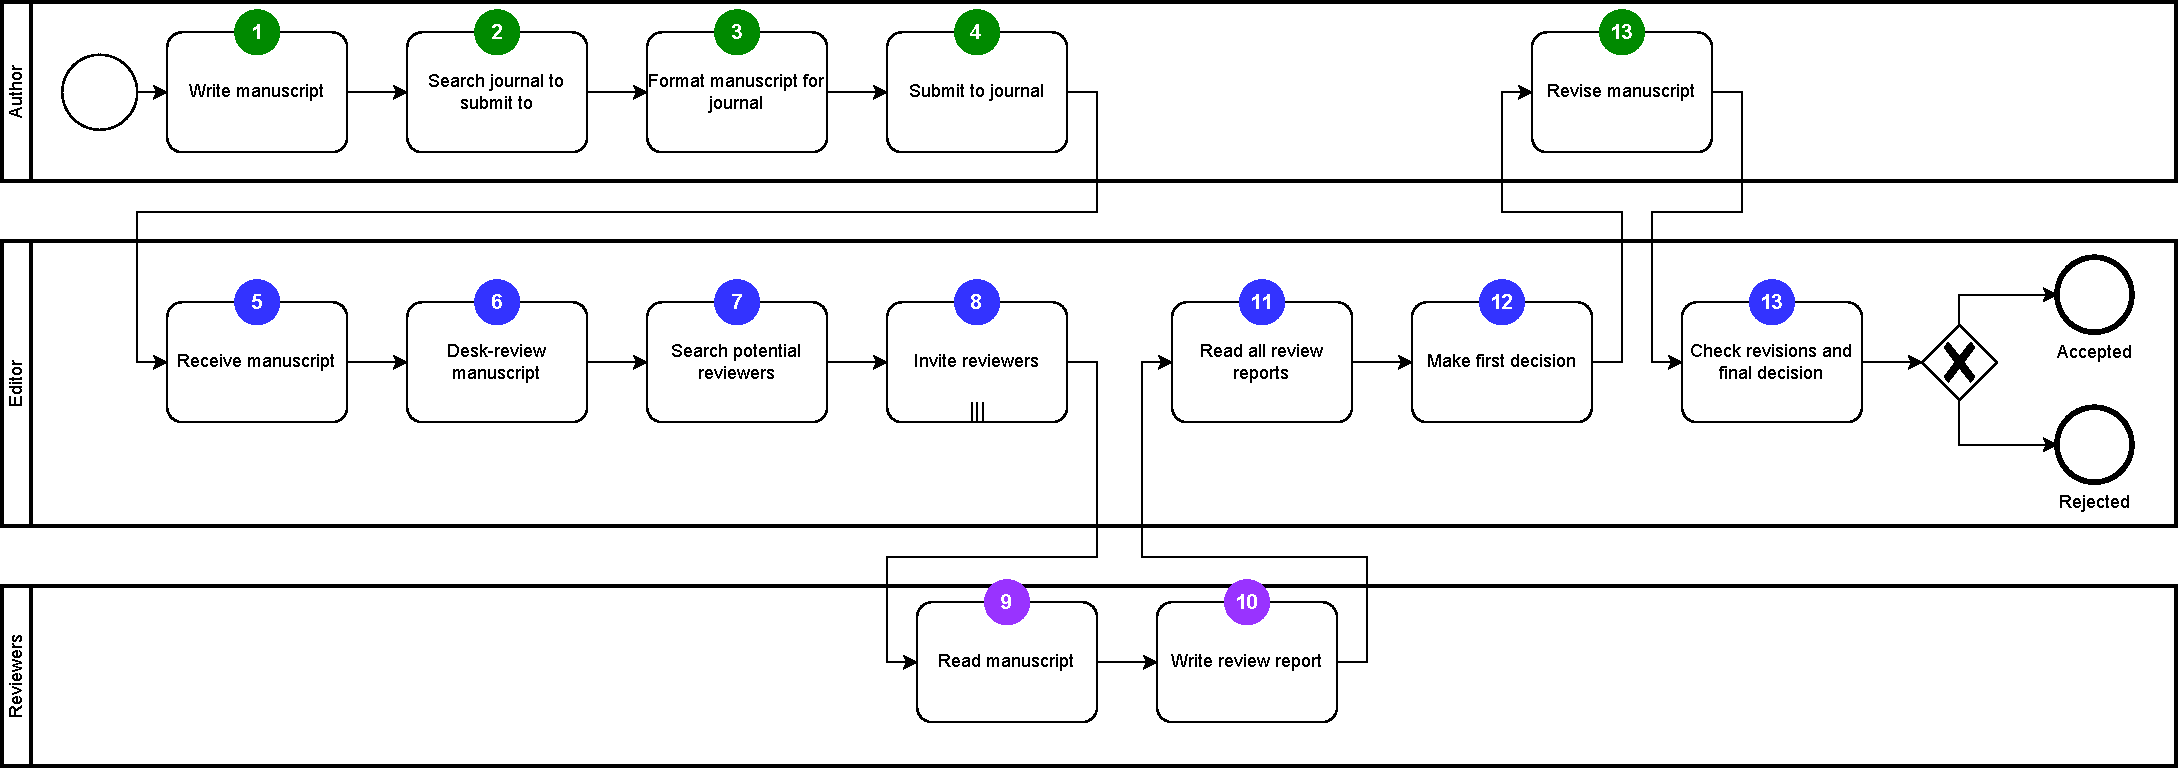
\includegraphics[width=\linewidth]{editorial_process.pdf}
        \caption{A simplified, typical editorial process from writing the manuscript to the final decision of acceptance or
        rejection for publication (in BPMN 2.0). For better understanding, the process steps performed by outside parties 
        are also modelled and the process starts with the outside party (author) writing the manuscript. The numbers
        indicate the sequence flow of the process.}
        \label{fig:bpmnEditorialProcess}
    \end{figure*}
\end{landscape}

\subsection{Use Cases For AI in the Editorial Process}

Table  ~\ref{tab:editorialProcess} shows an overview of the use cases for hybrid AI systems for each step in the typical editorial process.
{\color{purple} @todo: then we can pick those areas where adaptive hybrid AI could be interesting and reason why so\dots}


\subsection{Step XY}

{\color{purple} @todo: then we can pick exactly one adaptive hybrid AI use case, draw 1-2 hypotheses that we can research 
during the workshop\dots}


\begin{landscape}
    \begin{table}[htb]
        \caption{
            Typical editorial processing steps and use cases for (hybrid) AI for a scholarly journal.
        }
        \label{tab:editorialProcess}

        \tiny
        \renewcommand{\arraystretch}{1.1}
        \small\centering
        \setlength\tabcolsep{8pt}
        \begin{tabularx}{\linewidth}{s m l X X}
            \toprule
            \textbf{Step} & \textbf{Role} & \textbf{Task} & \textbf{AI Use Cases} & \textbf{Adaptability Aspect} \\
            \midrule

            \circled{1} & Author & Writes manuscript & 
                Literature search, literature recommendation, summarization of key findings, writing (auto-completion), translating, grammar and spell-checking &
                AI adapts to user by learning what papers are relevant, recommends more similar papers, and expands to related concepts. \linebreak
                AI suggests auto-completions and corrections based on the \textit{user's writing style} and the context of the manuscript.
                \\ 

            \circled{2} & Author & Searches for journals to submit to & Journal recommendation &
                AI adapts to user by learning what journals are relevant to the user (journals read / cited, and journals previously published in)
                and recommends more similar journals.
                \\

            \circled{3} & Author & Formats paper to meet journal's requirements & Manuscript conversion and styling & 
                AI learns styles of journals and adapts its output to the journal selected by user \\

            \circled{4} & Author & Submits paper to a journal & Extraction of metadata & (Adaptability not required) \\

            \circled{5} & Editor & Receives manuscript submission & Summarization of key findings & (Adaptability not required) \\
            
            \circled{6} & Editor & Conducts desk review of the manuscript & Checks of the manuscript, including detecting plagiarism, tortured phrases
                ("paraphrased plagiarism"), generated papers, biased or inappropriate language, off-topic references, fabricated or manipulated images,
                potentially inappropriate authorship, controversial topics, etc. & AI needs to adapt to recent literature (e.g., plagiarism check needs
                to account for latest literature) and detecting new methods of generating papers.\\ 

            \circled{7} & Editor & Searches for potential reviewers & Semantic search (in vector space using word embeddings), graph embeddings,
                review assignment algorithms using e.g., knowledge graph to exclude potential reviewers with conflicts of interest & AI needs to
                adapt to recent literature and previous reviewer preferences of the editor \\ 

            \circled{8} & Editor & Invites potential reviewers to review & E-mail writing, generate summary of the manuscript &
                AI should learn the user's writing style and typical wording from previous examples. \\

            \circled{9} & Reviewer & Reads the manuscript & Summarization of key findings, checking of the content of cited references &
                AI needs to adapt to recent cited literature. \\ 

            \circled{10} & Reviewer & Writes review report & Writing (auto-completion) of qualitative review report: help reviewer to avoid biases,
                inappropriate feedback, lack of specificity & (Adaptability not required) \\ 

            \circled{11} & Editor & Reads all review reports & Checking of the quality of the peer-review report: detect biases, inappropriate 
                language, generic / non-specific feedback, ad hominem criticism, off-topic comments, etc.  & (Adaptability not required) \\ 

            \circled{12} & Editor & Makes decision on manuscript & Summarization of peer-review outcome for decision letter
                to author & AI should learn the user's writing style and typical wording from previous examples. \\ 

            \circled{13} & Author & Revises manuscript & Checking that reviewer concerns are being addressed, writing (auto-completion) of
                rebuttal letter to the reviewers \& editors & AI should learn the user's writing style and typical wording from previous examples. \\
                
            \bottomrule
        \end{tabularx}
    \end{table}
\end{landscape}


